\chapter{Κωδικοποιητής κίνησης}
\label{ch:encoder}

Προκειμένου να παρέχεται στο μικροελεγκτή μία ένδειξη για την πορεία της κίνησης
του κάθε κινητήρα, κρίνεται σκόπιμη η ύπαρξη μίας μορφής ανατραφοδότησης· ενός
αισθητήρα που παρακολουθεί κάποιο φυσικό φαινόμενο που σχετίζεται με την κίνηση
του κινητήρα (βλ. σχήμα \ref{fig:encoder:lvl-0}).

\begin{figure}
    \caption{Επίδραση και ανάδραση μικροελεγκτή και κινητήρα.
    \label{fig:encoder:lvl-0}}
    \begin{center}
    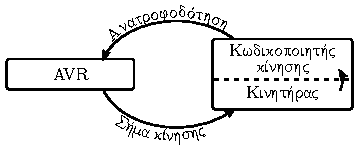
\includegraphics{encoder_lvl-0}
    \end{center}
\end{figure}

Παρότι υπάρχουν διάφορα φαινόμενα που μπορούν να χρησιμοποιηθούν για αυτόν το
σκοπό (όπως μαγνητισμός, ηλεκτρική αντίσταση σε μορφή ποτενσιόμετρου),
επιλέγεται η χρήση των, πλέον ίσως όχι και τόσο διαδεδομένων, υπερύθρων ακτίνων.
Το επιδιωκόμενο αποτέλεσμα παρουσιάζεται στο σχήμα \ref{fig:encoder:lvl-1}.

Όπως φαίνεται στο σχήμα, ο αισθητήρας αποτελείται από έναν πομπό και ένα δέκτη
υπερύθρων ακτίνων (φωτοδίοδος και φωτοτρανζίστορ, αντίστοιχα).
Η άτρακτος είναι ο άξονας περιστροφής του κινητήρα. Πάνω σε αυτόν προσκολλάται
μία ειδικά σχεδιασμένη ταινία, η οποία καθώς περιστρέφεται ως αποτέλεσμα
περιστροφής της ατράκτου, επηρεάζει την ένταση των εκπεμπόμενων ακτίνων του
πομπού που καταφθάνουν στο δέκτη, η οποία, με τη σειρά της, επηρεάζει την ένταση
της εξόδου του. Με αυτόν τον τρόπο επιτυγχάνεται η μετατροπή την στροφικής
κίνησης σε ηλεκτρικούς παλμούς οι οποίοι επιστρέφονται, ιδανικά, ως τετραγωνικοί
παλμοί.

\begin{figure}
    \caption{Σχηματική απεικόνιση κωδικοποιητή υλοποίησης.
    \label{fig:encoder:lvl-1}}
    \begin{center}
    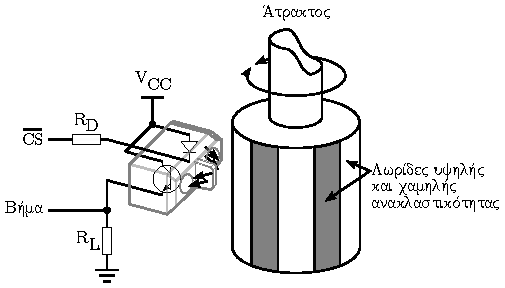
\includegraphics{encoder_lvl-1}
    \end{center}
\end{figure}

Ο αυτοσχέδιος κωδικοποιητής της υλοποίησης πρόκειται για έναν προσαυξητικό
κωδικοποιητή, δηλαδή του οποίου η έξοδος πληροφορεί για την πραγματοποίηση ενός
μικρού βήματος από μία λωρίδα στην επόμενη.
Σε σχέση με τους απόλυτους κωδικοποιητές που πληροφορούν τη συγκεκριμένη θέση
(πιθανώς, σε μοίρες) στην οποία βρίσκεται η άτρακτος, έχει το πλεονέκτημα ότι
είναι πολύ πιο απλός στην υλοποίηση και τη διασύνδεση με το μικροελεγκτή, καθώς
απαιτεί μόνο έναν αισθητήρα και, συνεπώς, μία γραμμή σύνδεσης για κάθε κινητήρα.
Περισσότερα αναφέρονται στην ενότητα \nameref{subsec:encoder:output} (σ.~%
\pageref{subsec:encoder:output}).

Ωστόσο, σε αντίθεση με τη συνήθη μορφή, η υλοποίηση χρησιμοποιεί μία ταινία που
εφάπτεται της ατράκτου αντί δίσκου. Η επιλογή αυτή γίνεται καθαρά για
διευκόλυνση της τοποθέτησης των εξαρτημάτων, παρά την ενδεχόμενη μείωση της
ακρίβειας του κωδικοποιητή.

Η επιλογή του υλικού της ταινίας, το πλάτος των λωρίδων της, η απόσταση και η
διάταξη (κάθετα ή παράλληλα) του αισθητήρα σε σχέση με αυτές καθώς και η γωνιακή
ταχύτητα της ατράκτου επηρεάζουν την ικανότητα αναγνώρισης των μεταβολών από τη
μία λωρίδα στην επόμενη (βλ. \nameref{subsec:reflex:coupling-factor} σ.~%
\pageref{subsec:reflex:coupling-factor}).
Επιπρόσθετα στοιχεία που επηρεάζουν την ακρίβεια του αισθητήρα και, για την
ακρίβεια, την πιθανότητα εσφαλμένης εξόδου από το δέκτη (φωτοτρανζίστορ) είναι
το αναφερόμενο ως ρεύμα ηρεμίας (\te{dark current}) και παρεμβολές από
περιβάλλουσες φωτεινές πηγές, καθώς και η θερμοκρασία εν γένει. Αυτές οι,
δευτερευούσης σημασίας, παράμετροι αναφέρονται στη σελίδα
\pageref{subsec:reflex:other-parameters}.

Στην ενότητα \nameref{subsec:reflex:calculations} (σ.~%
\pageref{subsec:reflex:calculations}) γίνεται μία προσπάθεια εκτίμησης των
ιδιοτήτων των στοιχείων που απαρτίζουν κάθε κωδικοποιητή ώστε να παραχθεί το
επιθυμητό αποτέλεσμα.
Μέρος αυτών των υπολογισμών αφιερώνεται στο προσδιορισμό της αντίστασης των
αντιστατών R\tsub{D} και R\tsub{L} του σχήματος, εκ των οποίων ο πρώτος ελέγχει
την ένταση που διαρρέει τη φωτοδίοδο, ενώ ο δεύτερος, χρησιμεύει για την
παραγωγή δύο διακριτών τιμών (λογικό 0 και 1) ως έξοδο του κωδικοποιητή.


\section{Οπτικοί κωδικοποιητές}
\label{sec:encoder:optical}

Σύμφωνα με έκδοση της \textcite[12]{drc76}, οπτικοί κωδικοποιητές περιστροφικής
κίνησης, παραδοσιακά, κατασκευάζονται με την προσάρτηση ενός περιφερειακά
διάτρητου δίσκου στον άξονα κίνησης εκατέρωθεν του οποίου διατάσσεται αντικριστό
ζεύγος πομπού και δέκτη υπέρυθρων ακτίνων. Καθώς ο δίσκος περιστρέφεται ως
αποτέλεσμα κίνησης του άξονα, η ύπαρξη ή έλλειψη οπής επαναφέρει ή αποκόπτει την
επικοινωνία μεταξύ πομπού-δέκτη προκαλώντας εναλλαγές στην έξοδο του δέκτη
\parencite[12]{drc76}.

\begin{figure}
    \caption{Προσαυξητικός οπτικός κωδικοποιητής με χρήση φωτοδιακόπτη.
    \label{fig:encoder:incremental}}
    \begin{center}
    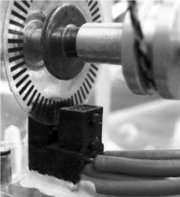
\includegraphics{encoder_incremental}
    \end{center}
    \fullcite{tycho:incremental}
\end{figure}


\subsection{Αναγνώριση θέσης}
\label{subsec:encoder:output}

\subsubsection{Προσαυξητικοί}

Στην απλούστερη υλοποίηση, ο αισθητήρας αναγνωρίζει τη μετάβαση από τη μία θέση
στην επόμενη ενώ είναι αδύνατο να αναχθεί από το σήμα και μόνον, είτε η φορά
περιστροφής είτε η τρέχουσα γωνιακή μετατόπιση του άξονα· ο ελεγκτής είναι
υπεύθυνος για την εξαγωγή αυτών των συμπερασμάτων \parencites[5--6]{lynch02}
[13]{drc76}. Στην περίπτωση αυτή, ο κωδικοποιητής αποκαλείται
προσαυξητικός\index{προσαυξητικός κωδικοποιητής} (incremental)
\parencite[5]{lynch02}. Ένα παράδειγμα προσαυξητικού κωδικοποιητή περιστροφικής
κίνησης παρουσιάζεται στην εικόνα \ref{fig:encoder:incremental}.


\subsubsection{Απόλυτης θέσης}

Ωστόσο, είναι δυνατό να κατασκευαστεί απόλυτος (absolute)
κωδικοποιητής\index{κωδικοποιητής απόλυτης μετατόπισης} μετατόπισης, κάνοντας
χρήση πολλαπλών ζευγών πομπού-δέκτη και ενός δίσκου υποδιαιρεμένου σε διακριτές
θέσεις που αποτελούνται από μοναδικό συνδυασμό οπών \parencites[6]{lynch02}. Ο
κάθε αισθητήρας παράγει έξοδο ανεξάρτητη από τους υπολοίπους βάσει των οπών που
του αντιστοιχούν, ενώ η συνδυαστική έξοδος όλων των αισθητήρων περιγράφει τον
τρέχοντα συνδυασμό οπών και συνεπώς τη γωνιακή μετατόπιση του δίσκου
\parencites[6]{lynch02}.


\subsection{Διάταξη στοιχείων}
\label{subsec:encoder:layout}

Για τη σύνθεση ενός κωδικοποιητή που κάνει χρήση οπτικών αισθητήρων,
χρησιμοποιούνται ζεύγη πομπού και δέκτη υπέρυθρων ακτίνων. Το κάθε ζεύγος μπορεί
να αποτελείται από ανεξάρτητα, μεταξύ τους, στοιχεία ή να βρίσκονται
ενσωματωμένα σε ειδική θήκη που διευκολύνει την τοποθέτησή τους (όπως στην
περίπτωση της εικόνας \ref{fig:encoder:incremental}).


\subsubsection{Φωτοδιακόπτες}

Υπάρχουν διατάξεις που τοποθετούν αντικριστά το ζεύγος πομπού και δέκτη
σχηματίζοντας έναν κενό χώρο μεταξύ τους στον οποίο μπορεί να εισέρχεται
εξωτερικό αντικείμενο, διακόπτοντας την επικοινωνία τους. Τέτοιοι αισθητήρες
αναφέρονται ως φωτοδιακόπτες\index{φωτοδιακόπτης}
(photointerrupter) \parencite[3]{lynch02} και αποτελούν τη διάταξη που
έχει παρουσιαστεί μέχρι τώρα.


\subsubsection{Ανακλαστικοί}

Σε εναλλακτική διάταξη, πομπός και δέκτης είναι μεταξύ τους παρακείμενοι με την
επικοινωνία τους να είναι δυνατή μόνο εφόσον οι εκπεμπόμενες ακτίνες ανακλαστούν
σε εξωτερική επιφάνεια (σχήμα \ref{fig:reflex:tct5000}).
Τέτοιοι αισθητήρες αναφέρονται ως ανακλαστικοί \index{ανακλαστικός αισθητήρας}
(reflective) \parencite[3]{lynch02}.
Η έξοδος του δέκτη επηρεάζεται άμεσα από την ένταση των προσπίπτουσων ακτίνων η
οποία, με τη σειρά της, εξαρτάται από τις ανακλαστικές ιδιότητες και την
απόσταση της εξωτερικής επιφάνειας \parencite{vishay06}.

Για την κατασκευή
οπτικού κωδικοποιητή κάνοντας χρήση αισθητήρα τέτοιας διάταξης, ο προσαρτημένος
στον άξονα περιστροφής δίσκος είναι χωρισμένος σε τμήματα διαφορετικού και
εναλλασσόμενου συντελεστή ανάκλασης ώστε με την περιστροφή του να επηρεάζεται η
ένταση των προσπίπτουσων ακτίνων στον κάθετο ως προς το δίσκο αισθητήρα, και,
συνεπώς, η έξοδός του \parencite[11]{vishay02}.


\section{Ανακλαστικός αισθητήρας TCRT5000}

\begin{figure}
    \caption{Ο ανακλαστικός οπτικός αισθητήρας TCRT5000.
    \label{fig:reflex:tcrt5000}}
    \begin{center}
    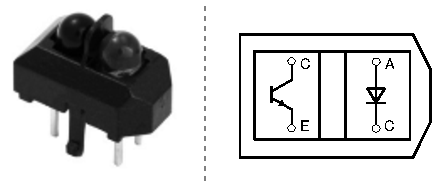
\includegraphics{reflex_tcrt5000}
    \end{center}
    \fullcite{vishay09:tcrt5000}
\end{figure}

Η ενότητα ασχολείται με τις διάφορες παραμέτρους που επηρεάζουν την απόδοση ενός
ανακλαστικού αισθητήρα προκειμένου να προσδιοριστούν οι απαιτήσεις για τη
συνδεσμολογία του με το μικροελεγκτή και την τοποθέτησή του σε σχέση με τους
κινητήρες με γνώμονα την κάλυψη των αναγκών για την παρακολούθηση της κίνησης
των τελευταίων.

Στην περίπτωση του συγκεκριμένου αισθητήρα, TCRT5000, ο δέκτης πρόκειται για ένα
φωτοτραζίστορ· ένα φωτοευαίσθητο ημιαγωγό όπου η ένταση διέλευσης ρεύματος
μεταξύ συλλέκτη (\te{collector}) και εκπομπού (\te{emitter}) ελέγχεται από την
ένταση των προσπίπτουσων ακτίνων, ενώ ο πομπός, μία φωτοδίοδος· ένα ημιαγωγό που
προκαλεί την παραγωγή φωτός (στην προκειμένη υπέρυθρου) όταν διαρρέεται από
ρεύμα. Όπως φαίνεται και στο σχήμα \ref{fig:reflex:tcrt5000}, τα δύο στοιχεία
(φωτοδίοδος και φωτοτρανζίστορ) είναι απομονωμένα μεταξύ τους από ένα ενδιάμεσο
τοίχωμα. Η επικοινωνία τους καθίσταται δυνατή μόνο εφόσον τα πλησιάσει εξωτερικό
αντικείμενο.


\subsection{Συντελεστής σύζευξης}
\label{subsec:reflex:coupling-factor}

Σύμφωνα με τη \textcite{vishay02}, στους ανακλαστικούς αισθητήρες που κάνουν
χρήση φωτοτρανζίστορ, ο λόγος της έντασης ρεύματος του συλλέκτη προς το ρεύμα
ορθής φοράς, $\frac{I_{C}}{I_{F}}$, αναφέρεται ως συντελεστής σύζευξης
\index{συντελεστής σύζευξης} (coupling factor), $k$, και περιγράφει το
βαθμό οπτικής σύνδεσης μεταξύ πομπού και δέκτη.
Ο προσδιορισμός του γίνεται για ορισμένη ανακλαστική επιφάνεια και απόσταση από
αυτήν και επηρεάζεται από την ένταση ρεύματος του πομπού, τη θερμοκρασία και τη
συχνότητα εναλλαγής μεταξύ επιφανειών διαφορετικών συντελεστών ανάκλασης
\parencite{vishay02}.


\subsubsection{Ανακλαστική επιφάνεια}

Ο πίνακας \ref{tab:reflex:materials}, ο οποίος αποτελεί απόσπασμα μετρήσεων της
\textcite{vishay06},
παρουσιάζει το ποσοστό της έντασης ρεύματος που σημειώνεται στο συλλέκτη για
διάφορα ανακλαστικά υλικά σε σχέση με τη χρήση της λευκής όψης κάρτας Kodak
neutral (No\@.Q-13).
Για τις ανάγκες της υλοποίησης, η επιφάνεια κωδικοποίησης είναι αρκετό να
αποτελείται από διαδοχικά τμήματα που παρουσιάζουν μεγάλη απόκλιση στους
συντελεστές ανάκλασης, ώστε να μην παρατηρείται επικάλυψη στο εύρος έντασης
ρεύματος του συλλέκτη για καθένα και, συνεπώς, να αυξάνεται η δυνατότητα
διάκρισή τους. Μία δεύτερη απαίτηση είναι η διαθεσιμότητα και η ευχρηστία των
αντίστοιχων υλικών ώστε να είναι άμεση η ενδεχόμενη αντικατάσταση ή τροποποίηση
της επιφάνειας κωδικοποίησης.

\begin{table}
\caption{Σχετική απόδοση διάφορων ανακλαστικών υλικών.
\label{tab:reflex:materials}}

Σε όλες τις μετρήσεις, το ρεύμα
ορθής φοράς, $I_{F}$, ήταν σταθερό στα 20mA, ο αισθητήρας τοποθετημένος κάθετα
ως προς την ανακλαστική επιφάνεια σε απόσταση όπου ο συλλέκτης αποδίδει τη
μέγιστη έξοδο για υπέρυθρες των 950nm \textcite{vishay06}.\\~

\begin{tabu} to \linewidth{X X[-1,R] X[-1] X X[-1,R]}
\multicolumn2{l}{\bfseries Kodak neutral card}    & &
\multicolumn2{l}{\bfseries Black on white typewritting paper} \\
\cline{1-2}\cline{4-5}

White side (reference medium)           &   100\%   & &
Drawing ink (Higgins, Pelikan)          &   4--6\%  \\

Gray side                               &   20\%    & &
Foil ink (Rotring)                      &   50\%    \\

\multicolumn2{l}{\bfseries Paper}                   & &
Fiber-tip pen (Edding 400)              &   10\%    \\
\cline{1-2}

Typewriting paper                       &   94\%    & &
Fiber-tip pen, black (Stabillo)         &   76\%    \\

Drawing card, white (Schoeller)         &   100\%   & &
Photocopy                               &   7\%    \\

Card, light gray                        &   67\%    & &
\multicolumn2{l}{\bfseries Plotter pen}             \\
\cline{4-5}

Envelope (beige)                        &   100\%   & &
HP fiber-tip pen (0.3mm)               &   84\%     \\

Packing card (light brown)              &   84\%    & &
Black 24 needle printer                 &   28\%    \\

Newspaper paper                         &   97\%    & &
Ink (Pelikan)                           &   100\%   \\

Pergament paper                         &   30--42\% & &
Pencil, HB                              &   26\%    \\
\end{tabu}

\floatfoot{\fullcite[2]{vishay06:materials}}
\end{table}

Με αυτά τα κριτήρια, επιλέγεται το απλό τυπογραφικό χαρτί ως επιφάνεια υψηλού
συντελεστή ανάκλασης (94\%) με την επικάλυψη του με φωτοτυπικό μελάνι ως
επιφάνεια χαμηλού συντελεστή (7\%).

Για περαιτέρω απλούστευση της υλοποίησης, επιλέγεται η αντικατάσταση του δίσκου
κωδικοποίησης με ταινία η οποία καλύπτει την περιφέρεια του άξονα περιστροφής
στο σημείο όπου είναι τοποθετημένος ο αισθητήρας.

%Αναφορά σε πιθανές επιπτώσεις


\subsubsection{Λειτουργική απόσταση}

Η απόσταση του αισθητήρα από την ανακλαστική επιφάνεια επηρεάζει άμεσα το
ποσοστό των προσπίπτουσων ακτίνων στο δέκτη που είναι υπεύθυνες για τη διέγερση
του φωτοτρανζίστορ. Η απόσταση αυτή αποκαλείται λειτουργική απόσταση
\index{λειτουργική απόσταση} (operating distance), $d$, και, για μία
τυπική υλοποίηση, απεικονίζεται στο σχήμα \ref{fig:reflex:working-diagram}(αʹ)
\parencite{vishay02}.

Όπως είναι αναμενόμενο, καθώς η λειτουργική απόσταση μεταβάλλεται, η ένταση
ρεύματος του συλλέκτη αυξομειώνεται. Σύμφωνα με τη τον οδηγό της
\textcite{vishay06}, η σχέση αυτή απεικονίζεται στο λειτουργικό διάγραμμα
\index{λειτουργικό διάγραμμα} (operating diagram) στο εγχειρίδιο χρήσης
κάθε αισθητήρα.

Το σχήμα \ref{fig:reflex:working-diagram}(βʹ) αποτελεί το λειτουργικό διάγραμμα
του επιλεγμένου αισθητήρα, TCRT5000, όπου παρουσιάζεται η ένταση ρεύματος του
συλλέκτη, $I_{C}$, σε σχέση με τη μέγιστη δυνατή, $I_{Cmax}$, καθώς μεταβάλλεται
η λειτουργική απόσταση.
Επίσης, παρατηρείται ότι η μέγιστη ένταση του συλλέκτη, $I_{C} = I_{Cmax}$,
σημειώνεται για μία λειτουργική απόσταση $d = 2.5$cm.

\begin{figure}
    \caption{Λειτουργική απόσταση και λειτουργικό διάγραμμα.
        \label{fig:reflex:working-diagram}}
    \begin{center}
        \begin{subfigure}[b]{0.45\textwidth}
            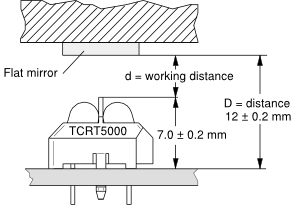
\includegraphics[width=0.95\textwidth]{reflex_test-circuit.png}
            \caption{}
        \end{subfigure}
        \begin{subfigure}[b]{0.45\textwidth}
            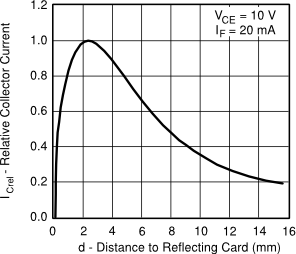
\includegraphics[width=0.9\textwidth]{reflex_working-distance.png}
            \caption{}
        \end{subfigure}
    \end{center}

    (αʹ): \fullcite[3]{vishay09:test-circuit}

    (βʹ): \fullcite[4]{vishay09:working-distance}
\end{figure}

Για τις ανάγκες της υλοποίησης, επιλέγεται λειτουργική απόσταση 2.5cm έτσι ώστε
ο συντελεστής σύζευξης να ευνοείται όσο το δυνατόν περισσότερο.


\subsubsection{Διάστημα εναλλαγής}

Για τις ανάγκες της υλοποίησης, ο άξονας περιστροφής επικαλύπτεται, στο ύψος του
αισθητήρα, από διαδοχικά τμήματα υψηλότερου και χαμηλότερου συντελεστή
ανάκλασης. Καθώς ο άξονας περιστρέφεται, η ένταση ρεύματος του συλλέκτη
μεταβάλλεται από τη μέγιστη μέχρι την ελάχιστη δυνατή και αντίστροφα.
Ωστόσο, σύμφωνα με το εγχειρίδιο της \textcite{vishay06}, εάν το πάχος των
τμημάτων είναι πολύ μικρό, ενδέχεται οι εναλλαγές να μην εκδηλώνονται αισθητά
στην ένταση ρεύματος του συλλέκτη.

Στο σχήμα \ref{fig:reflex:switching-distance} παρουσιάζεται η ένταση ρεύματος
του συλλέκτη για δύο διαδοχικά τμήματα.
Το σημείο εναλλαγής από τον ένα συντελεστή ανάκλασης στον επόμενο σημειώνεται
με το $Xo$ ενώ με $I_{c1}$ και $I_{c2}$, η μέγιστη ένταση ρεύματος του
συλλέκτη όταν η κοινή επιφάνεια $g$ των οπτικών πεδίων πομπού και δέκτη
καλύπτεται πλήρως από τμήμα του αντίστοιχου συντελεστή.
Προκύπτει ότι, ενώ η μετάβαση από τον ένα συντελεστή στον επόμενο συμβαίνει
ακαριαία, η ένταση ρεύματος του συλλέκτη $I_C$ έχει αρχίσει να μειώνεται σε
προγενέστερη μετατόπιση, όταν ένα πρώτο τμήμα των αρχικά διαθέσιμων ακτίνων
αποκόπηκε από το δέκτη, και συνεχίζει να μειώνεται σταδιακά έως ότου το τμήμα με
το νέο συντελεστή έχει καλύψει πλήρως την περιοχή $g$.

\begin{figure}
    \caption{Σχέση μεταβολής ρεύματος $I_C$ και συντελεστή ανάκλασης.
        \label{fig:reflex:switching-distance}}
    \begin{center}
        \begin{subfigure}{0.45\linewidth}
            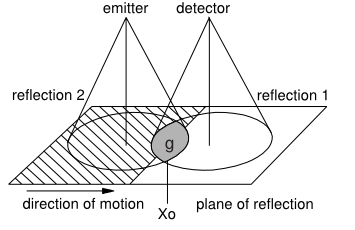
\includegraphics{reflex_switching-distance_a.png}
        \end{subfigure}
        \begin{subfigure}{0.45\linewidth}
            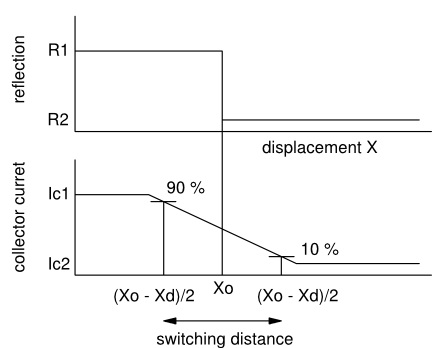
\includegraphics{reflex_switching-distance_b.png}
        \end{subfigure}
    \end{center}
    \fullcite[3]{vishay06:switching-distance}
\end{figure}

Επίσης, συμπεραίνεται ότι, καθώς το πάχος των τμημάτων μειώνεται ώστε η περιοχή
$g$ να είναι αδύνατο να καλυφθεί εξ ολοκλήρου από ένα μόνο τμήμα, η μέγιστη και
ελάχιστη τιμή έντασης ρεύματος που είναι δυνατό να σημειωθούν αρχίζουν να
συγκλίνουν, εφόσον, πλέον, σε κάθε μετατόπιση καταφθάνουν στο δέκτη ακτίνες από
όλο και περισσότερα τμήματα.

Το ελάχιστο πάχος τμημάτων καθορίζεται από το διάστημα εναλλαγής\index{διάστημα%
εναλλαγής} (switching distance),
$X_d$, το οποίο ορίζεται ως το διάστημα μεταξύ δύο διαδοχικών τμημάτων
διαφορετικών συντελεστών ανάκλασης στο οποίο παρατηρείται το 90\% $I_{C_1}$ έως
το 10\% $I_{C2}$ \parencite{vishay06}. Η τιμή του διαστήματος εναλλαγής
εξαρτάται, από την κατασκευή του αισθητήρα καθώς και τη λειτουργική απόσταση,
ενώ όσο πιο μικρή απόσταση εναλλαγής υποστηρίζει κάποιος αισθητήρας, τόσο
υψηλότερη η διακριτική ικανότητά (resolution) του
\parencites{vishay02}{vishay06}. Για τον αισθητήρα TCRT5000, το διάστημα
εναλλαγής ανέρχεται στα 1.9mm \parencite{vishay02}.

Στο σχήμα \ref{fig:reflex:d_switching-distance} παρουσιάζεται πώς η λειτουργική
απόσταση του αισθητήρα επηρεάζει το διάστημα εναλλαγής του. Οι εμφανιζόμενες
καμπύλες αποτελούν ένα κατώτατο όριο και αντιστοιχούν σε δύο διαφορετικούς
τρόπους τοποθέτησης του αισθητήρα σε σχέση με την ανακλαστική επιφάνεια.
Στη θέση~1, ο νοητός άξονας που ορίζεται από πομπό και δέκτη του αισθητήρα είναι
κάθετος ως προς τα εναλλασσόμενα τμήματα, ενώ στη θέση~2, παράλληλος.
Παρατηρείται ότι η θέση~1 υπερτερεί της θέσης~2 καθώς για την ίδια λειτουργική
απόσταση επιτυγχάνεται υψηλότερη διακριτική ικανότητα και, συνεπώς, προσφέρεται
υψηλότερο ελάχιστο διάστημα εναλλαγής. Δεδομένου ότι οι συνθήκες (ανάγκες και
περιορισμοί) το επιτρέπουν, επιλέγεται η θέση~1 για την υλοποίηση.

\begin{figure}
    \caption{Σχέση Λειτουργικής απόστασης και Διαστήματος εναλλαγής.
    \label{fig:reflex:d_switching-distance}}
    \begin{center}%
    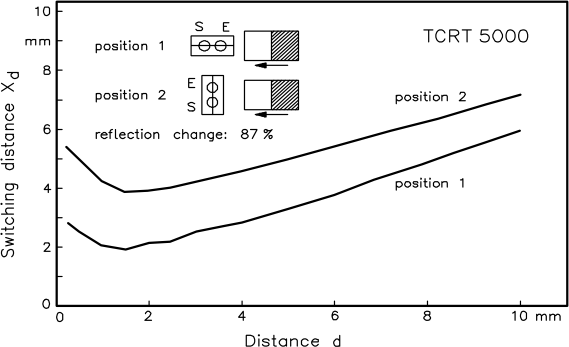
\includegraphics[width=0.7\textwidth]{reflex_d_switching-distance.png}%
    \end{center}

    \fullcite[8]{vishay02:d_switching-distance}
\end{figure}


\subsubsection{Συχνότητα αποκοπής}

Το φωτοτρανζίστορ---το πιο αργό στοιχείο του αισθητήρα---απαιτεί κάποιο χρόνο
για να ανταποκριθεί στις απότομες εναλλαγές έντασης των προσπίπτουσων ακτίνων
\parencite{vishay06}. Ως αποτέλεσμα, εάν οι νέες εναλλαγές προκύπτουν προτού η
έξοδος του να έχει κατασταλάξει για μία προηγούμενη εναλλαγή, τότε η αναγνώρισή
τους καθίσταται μάλλον αβέβαιη. Άμεση απόρροια αυτού, δηλαδή του χρόνου
απόκρισης του φωτοτρανζίστορ, είναι η ανάγκη προσδιορισμού μίας μέγιστης
επιτρεπόμενης συχνότητας εναλλαγής των τμημάτων διαφορετικού συντελεστή
ανάκλασης ώστε να μην επηρεάζεται δραματικά ο συντελεστής σύζευξης. Η συχνότητα
αυτή αναφέρεται ως συχνότητα αποκοπής \index{συχνότητα αποκοπής}
(cut-off frequency) και είναι η συχνότητα στην οποία παρατηρείται μείωση
περίπου 30\% του συντελεστή σύζευξης \parencite{vishay02}.

Το σχήμα \ref{fig:reflex:cutoff-frequency} παρουσιάζει πώς επηρεάζουν η τάση και
η αντίσταση φόρτου, $R_L$, του φωτοτρανζίστορ τη συχνότητα αποκοπής του
αισθητήρα.
Θα μπορούσε να χρησιμοποιηθεί χαμηλή τιμή αντίστασης φόρτου, ώστε να
μειωθεί ο χρόνος απόκρισης και, ως επέκταση, να διευρυνθεί το όριο της
συχνότητας αποκοπής. Ωστόσο, μία τέτοια κίνηση θα είχε ως αποτέλεσμα τη
μείωση της τάσης του παραγόμενου σήματος \parencite{vishay06}.
Προτιμάται να χρησιμοποιηθούν οι απαιτήσεις της υλοποίησης, όπως μέγιστη
ταχύτητα περιστροφής, για τον προσδιορισμό της συχνότητας αποκοπής και, μέσω
αυτής, της αντίστασης φόρτου.

\begin{figure}
    \caption{Σχέση Συχνότητας αποκοπής και Αντίστασης φόρτου.
    \label{fig:reflex:cutoff-frequency}}
    \begin{center}%
    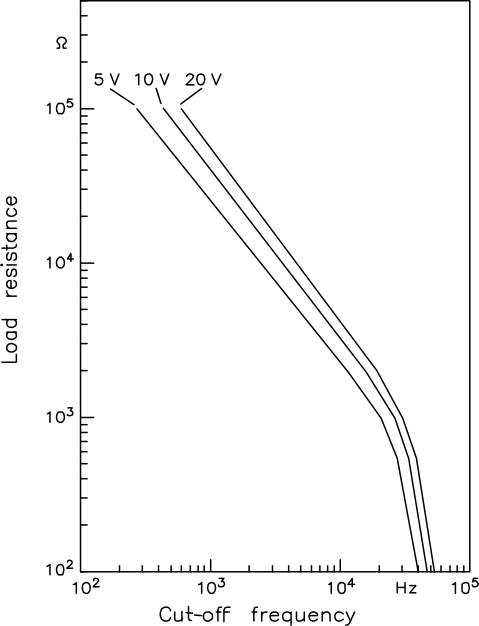
\includegraphics[width=0.5\textwidth]{reflex_cutoff-frequency.png}
    \end{center}

    \fullcite[5]{vishay02:cutoff-frequency}
\end{figure}


\subsubsection{Θερμοκρασία}
Η αύξηση θερμοκρασίας επηρεάζει την απόδοση τόσο της διόδου εκπομπής υπερύθρων,
η οποία μειώνεται, όσο και του φωτοτρανζίστορ, η οποία αυξάνεται
\parencite{vishay06}. Ωστόσο, όπως προκύπτει από το σχήμα
\ref{fig:reflex:t-amb_ctr-rel}, για θερμοκρασίες από 0°C έως 90°C, το
συνολικό αποτέλεσμα επηρεάζεται ελάχιστα. Θα μπορούσε, είτε να αγνοηθεί
πλήρως είτε να συμπεριληφθεί ως σταθερή μείωση του σχετικού λόγου μεταφοράς
ρεύματος.

\begin{figure}
    \caption{Σχέση θερμοκρασίας και Σχετικού λόγου μεταφοράς ρεύματος.
    \label{fig:reflex:t-amb_ctr-rel}}
    \begin{center}%
    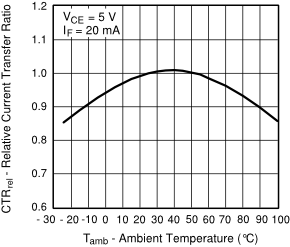
\includegraphics[width=0.5\textwidth]{reflex_t-amb_ctr-rel.png}
    \end{center}

    \fullcite[3]{vishay09:test-circuit}
\end{figure}


\subsubsection{Ένταση πομπού}

Η ένταση των εκπεμπόμενων ακτίνων εξαρτάται από κάποια χαρακτηριστικά κατασκευής
του αισθητήρα (όπως φακός εστίασης) και την ένταση ρεύματος της διόδου
υπερύθρων.
Αφενός, η δίοδος πρέπει να διαρρέεται από ρεύμα ορθής φοράς ελάχιστης έντασης
5mA ώστε να σταθεροποιείται η έξοδός της, αφετέρου, να μην ξεπερνά τη μέγιστη
αποδεκτή τιμή \parencite{vishay02}. Σύμφωνα με τις απόλυτες μέγιστες τιμές του
αισθητήρα TCRT5000, η μέγιστη ένταση ρεύματος ορθής φοράς, $I_F$, είναι 60mA, σε
θερμοκρασία περιβάλλοντος χώρου, $T_{amb}$, 25°C \parencite{vishay09}.

Παρόλο που η εφαρμογή της μέγιστης δυνατής έντασης παρέχει ισχυρότερο σήμα στο
δέκτη λόγω του υψηλότερου συντελεστή σύζευξης (σχήμα \ref{fig:reflex:i-f_ctr})
προτιμάται η εφαρμογή κατά πολύ χαμηλότερης. Στους λόγους συγκαταλέγεται η
τήρηση αποδεκτής έντασης ρεύματος σε περιβάλλον κυμαινόμενης θερμοκρασίας κυρίως
για την επιμήκυνση της διάρκειας ζωής του πομπού. Επίσης, στο ίδιο σχήμα
παρατηρείται ότι ο συντελεστής σύζευξης πλησιάζει ένα ανώτατο όριο 6\% για ρεύμα
ορθής φοράς στο εύρος 35--60mA. Επομένως, επιλέγεται να χρησιμοποιηθεί ρεύμα
ορθής φοράς έως και 35mA.

\begin{figure}
    \caption{Σχέση Ρεύματος ορθής φοράς και Λόγου μεταφοράς ρεύματος.
    \label{fig:reflex:i-f_ctr}}
    \begin{center}%
    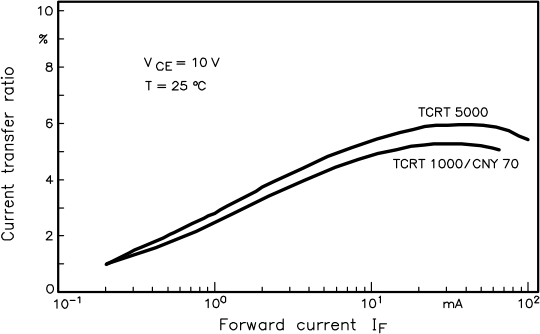
\includegraphics[width=0.8\textwidth]{reflex_i-f_ctr.png}
    \end{center}

    \fullcite[5]{vishay02:forward-current_ctr}
\end{figure}


\subsection{Λοιπές παράμετροι}
\label{subsec:reflex:other-parameters}


\subsubsection{Ρεύμα ηρεμίας}

Ένα φωτοτρανζίστορ διαρρέεται από ρεύμα ακόμα και όταν αυτό βρίσκεται πλήρως
απομονωμένο από φωτεινές πηγές. Το ρεύμα αυτό αναφέρεται ως ρεύμα ηρεμίας
\index{ρεύμα ηρεμίας} (dark current) και επηρεάζεται από την τιμή της
τάσης συλλέκτη-εκπομπού, $V_{CE}$, και, σε μεγαλύτερο βαθμό, από τη θερμοκρασία
\parencite{vishay06}. Τυπική τιμή ρεύματος ηρεμίας, $I_{CEO}$, για τον αισθητήρα
TCRT5000 είναι τα 10nA στα 20V \parencite{vishay09}.

Κρίνεται σκόπιμο να αγνοηθεί στο σχεδιασμό εφόσον προκύψει από τους υπολογισμούς
ότι το ρεύμα ηρεμίας έντασης περίπου 5μA που προκαλείται από την εφαρμογή
τάσης 10V σε μία οριακή θερμοκρασία, $T_{amb}$, 100°C, επηρεάζει ελάχιστα την
έξοδο του αισθητήρα (σχήμα \ref{fig:reflex:t-amb_i-ceo}).

\begin{figure}
    \caption{Σχέση θερμοκρασίας και Ρεύματος ηρεμίας.
    \label{fig:reflex:t-amb_i-ceo}}
    \begin{center}%
    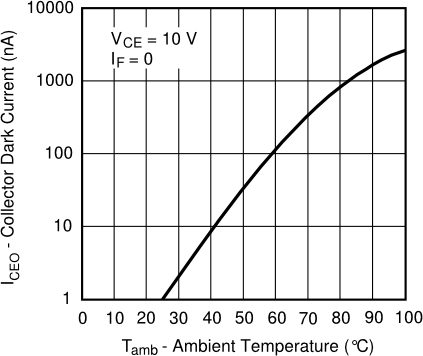
\includegraphics[width=0.5\textwidth]{reflex_t-amb_i-ceo.png}
    \end{center}

    \fullcite[3]{vishay06:dark-current}
\end{figure}


\subsubsection{Οπτικές παρεμβολές}

Σύμφωνα με τον οδηγό \textcite{vishay06}, είναι δυνατό να διοχετεύονται
εκπεμπόμενες ακτίνες από τον πομπό στο δέκτη απευθείας μέσα από την ίδια τη θήκη
καθώς και δια μέσω επιφανειών που περιβάλλουν τον αισθητήρα, πέραν της
ανακλαστικής επιφάνειας, με αποτέλεσμα να προκύπτει ένταση ρεύματος συλλέκτη.

Επιπλέον, σταθερή απευθείας πρόσπτωση φωτός στο φωτοτρανζίστορ μειώνει την
ευαισθησία του, δυνατό φως είναι δυνατό να το κρατήσει μονίμως ενεργό, ενώ
μεταβαλλόμενο, να προκαλέσει αδικαιολόγητη εναλλαγή στο σήμα εξόδου
\parencite{vishay06}.
Ο επιλεγμένος αισθητήρας διαθέτει προστατευτικά φίλτρα τα οποία παρεμποδίζουν το
ορατό φως \parencite{vishay09}. Ωστόσο, ένα μεγάλο εύρος του ηλιακού φωτός
αποτελείται από υπέρυθρες και, συνεπώς, η παράμετρος πρέπει να ληφθεί υπόψη κατά
το σχεδιασμό του συστήματος.

Η περίπτωση παρεμβολών που οφείλονται στην κατασκευή του αισθητήρα είναι δυνατό
να απαλειφθούν καταμετρώντας το σήμα του αισθητήρα σε πλήρη απομόνωσή του και
λαμβάνοντάς το υπόψη, ως σταθερά, κατά την κανονική λειτουργία του κωδικοποιητή.
Ο βαθμός στον οποίο επηρεάζουν οι περιβάλλουσες επιφάνειες μπορεί να εντοπιστεί
με παρόμοιο τρόπο. Ο βαθμός στον οποίο επηρεάζουν οι επικρατούσες συνθήκες
φωτισμού είναι, σαφώς, μεταβλητός και η ίδια προσέγγιση μη εφαρμοστέα. Ωστόσο,
είναι δυνατό να περιοριστεί απομονώνοντας εξωτερικά ολόκληρο τον κωδικοποιητή,
δηλαδή αισθητήρα και ανακλαστική επιφάνεια.


\subsubsection{Θερμοκρασία}

Σε προηγούμενη παράγραφο, μελετήθηκε πώς επηρεάζει η θερμοκρασία το συντελεστή
σύζευξης. Ωστόσο, η θερμοκρασία θέτει και ορισμένα άλλα ζητήματα προς μελέτη.

Η αύξηση θερμοκρασίας της διόδου, ως άμεσο υποπροϊόν της κατανάλωσης ισχύος,
παίζει καθοριστικό ρόλο στον προσδιορισμό της έντασης ρεύματος της διόδου.
Σύμφωνα με το εγχειρίδιο χρήσης τους αισθητήρα \parencite{vishay09}, η μέγιστη
επιτρεπτή τιμή ρεύματος ορθής φοράς του πομπού, $I_F$, ανέρχεται στα 60mA σε
θερμοκρασία περιβάλλοντος χώρου, $T_{amb}$, 25°C. Επιπλέον, καθώς η θερμοκρασία
αυξάνεται, το μέγιστο επιτρεπτό όριο μειώνεται.
Το σχήμα \ref{fig:reflex:power-dissipation} δίνει την απόλυτη μέγιστη τιμή
κατανάλωσης ισχύος σε σχέση με τη θερμοκρασία. Λαμβάνοντας υπόψη ότι $P = VI$,
είναι δυνατό να υπολογιστεί το μέγιστο επιτρεπτό ρεύμα ορθής φοράς βάσει των
διακυμάνσεων της θερμοκρασίας χώρου και της εφαρμοζόμενης τάσης της υλοποίησης.

\begin{figure}
    \caption{Σχέση Κατανάλωσης ισχύος και Θερμοκρασίας.
    \label{fig:reflex:power-dissipation}}
    \begin{center}%
    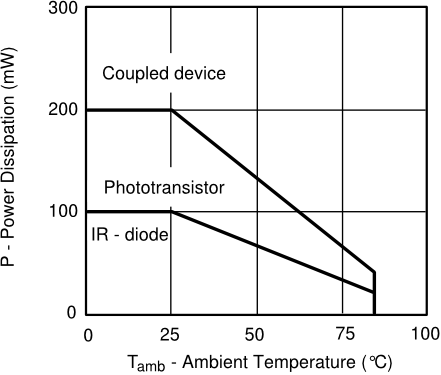
\includegraphics[width=0.5\textwidth]{reflex_power-dissipation.png}
    \end{center}

    \fullcite[3]{vishay09:power-dissipation}
\end{figure}

Κρίνεται αναγκαία η τήρηση χαμηλών θερμοκρασιών στη δίοδο για την επιμήκυνση της
ζωής της και, συνεπώς, του ίδιου του αισθητήρα, καθώς χαμηλή θερμοκρασία
συνεπάγεται ελάχιστη ή καθόλου φθορά της ένωσης p-n της διόδου. Προς επίτευξη
αυτού, η παρεχόμενη ένταση ρεύματος της διόδου είναι κατά πολύ μικρότερη από τη
μέγιστη αποδεκτή, κατάλληλη ακόμα και για θερμοκρασίες που ξεπερνούν τις
απαιτήσεις της υλοποίησης. Επίσης, ο αισθητήρας τίθεται σε λειτουργία μόνο για
τα διαστήματα περιστροφής του άξονα κίνησης, ώστε ο χρόνος κατανάλωσης ενέργειας
με αποτέλεσμα την εκπομπή θερμότητας και αύξηση της θερμοκρασίας τοπικά του
αισθητήρα να είναι περιορισμένος.


\subsection{Υπολογισμοί}
\label{subsec:reflex:calculations}


Σε αυτό το σημείο, επιχειρείται να προσδιοριστούν οι επακριβείς τιμές των
στοιχείων για τη σύνδεση του αισθητήρα υπέρυθρων και των τελικών προδιαγραφών
του κωδικοποιητή, λαμβάνοντας υπόψη τις παραμέτρους που έχουν ήδη περιγραφεί.

Μία βασική ανάγκη είναι η εκτίμηση της έντασης ρεύματος του συλλέκτη, ${I_C}$, η
οποία εξαρτάται από το ρεύμα ορθής φοράς, $I_F$, και το συντελεστή σύζευξης,
$k$.
\begin{equation}
I_C = k \cdot I_F \label{eq:reflex:i-c}
\end{equation}

Ο συντελεστής σύζευξης εξαρτάται από το ρεύμα ορθής φοράς και η σχέση τους
περιγράφεται από το σχήμα \ref{fig:reflex:i-f_ctr}. Ωστόσο, το σχήμα αυτό
αναφέρεται στη χρήση της
λευκής όψης κάρτας Kodak neutral σε λειτουργική απόσταση μέγιστης απόδοσης.

Στην υλοποίηση χρησιμοποιούνται διαφορετικά υλικά ως ανακλαστικές επιφάνειες
και, ενδεχομένως, διαφορετική λειτουργική απόσταση. Ο πραγματικός συντελεστής
σύζευξης για κάθε υλικό και λειτουργική απόσταση προκύπτει από την
\begin{equation}
k = I_{Crel} \cdot k_{Kodak} \label{eq:reflex:k}
\end{equation}
όπου $I_{Crel}$, η σχετική τιμή ρεύματος του συλλέκτη ως αποτέλεσμα του
ανακλαστικού υλικού, της λειτουργικής απόστασης και λοιπών παραμέτρων και
$k_{Kodak}$, ο συντελεστής σύζευξης με χρήση της κάρτας Kodak neutral.

%Προκειμένου να συνεχίσουν οι υπολογισμοί είναι απαραίτητο να επιλεγεί το ρεύμα
%ορθής φοράς.

Το ρεύμα ορθής φοράς, $I_F$, είναι επιθυμητό να επιλεγεί ώστε να μεγιστοποιείται
ο συντελεστής σύζευξης, $k$, και προκύπτει ότι για τον επιλεγμένο αισθητήρα,
TCRT5000, παρατηρείται για ρεύμα ορθής φοράς περίπου 35mA (σχήμα
\ref{fig:reflex:i-f_ctr}).
Ωστόσο, λαμβάνοντας υπόψη το σχήμα \ref{fig:reflex:power-dissipation} και την
ανάγκη για τήρηση χαμηλής κατανάλωσης ισχύος με εφαρμογή ορθής τάση
$V_F = 1.25$V στη δίοδο IR, αντί αυτού, επιλέγεται ρεύμα ορθής φοράς
\begin{equation}
I_F = 20\text{mA} \label{eq:reflex:i-f_value}
\end{equation}
με
\begin{equation}
k_{Kodak} = 5.5\% \label{eq:reflex:k_kodak-value}
\end{equation}

%Όπως προκύπτει από το σχήμα
%[\underline{REF}], %\ref{fig:reflex:ctr},
%για τον επιλεγμένο αισθητήρα, TCRT5000, ο μέγιστος λόγος μεταφοράς ρεύματος, ή
%συντελεστής σύζευξης, είναι 6\%. Ωστόσο, αναφέρεται στη χρήση της λευκής όψης
%κάρτας Kodak neutral, $k_{Kodak}$, σε λειτουργική απόσταση μέγιστης απόδοσης.

Έχει σημειωθεί ότι, εκτός και εάν προκύψει κάποια ιδιαίτερη ανάγκη, η
λειτουργική
απόσταση, $d$, του αισθητήρα επιλέγεται ώστε ο συντελεστής σύζευξης να ευνοείται
κατά το μέγιστο. Επομένως, από το σχήμα \ref{fig:reflex:working-diagram},
προκύπτει ότι
\begin{equation}
d = 2.5 \text{mm}
\end{equation}

Από το σχήμα \ref{fig:reflex:d_switching-distance} προκύπτει ότι για την
επιλεγμένη λειτουργική απόσταση (2.5mm), το ελάχιστο επιτρεπτό διάστημα
εναλλαγής είναι περίπου 2mm. Αφήνοντας περιθώριο σφάλματος, επιλέγεται διάστημα
εναλλαγής
\begin{equation}
X_d = 4 \text{mm}
\end{equation}

Στην υλοποίηση χρησιμοποιείται τυπογραφικό χαρτί ως επιφάνεια με υψηλό
συντελεστή σύζευξης, $k_H$, και φωτοτυπικό μελάνι ως επιφάνεια με χαμηλό
συντελεστή, $k_L$.
Λαμβάνοντας υπόψη τον πίνακα ανακλαστικών υλικών
(πίνακας \ref{tab:reflex:materials}), το
λειτουργικό διάγραμμα για απόσταση $d = 2.5$mm
(σχήμα \ref{fig:reflex:working-diagram}β) και τη σχέση
\eqref{eq:reflex:k_kodak-value}, αντικαθιστώντας στη σχέση \eqref{eq:reflex:k},
προκύπτει ότι
\begin{equation}
k_H = 94 \% \cdot 5.5 \% = 5.17 \%
\end{equation}
\begin{equation}
k_L = 7 \% \cdot 5.5 \% = 0.385 \%
\end{equation}

Με γνωστούς τους συντελεστές σύζευξης $k_H$ και $k_L$ των δύο επιφανειών και το
ρεύμα ορθής φοράς (σχέση \eqref{eq:reflex:i-f_value}), είναι πλέον δυνατός ο
υπολογισμός των αντίστοιχων τιμών της έντασης ρεύματος του συλλέκτη,
αντικαθιστώντας στη σχέση \eqref{eq:reflex:i-c}
\begin{equation}
I_{C_H} = 5.17\% \cdot 20 \text{mA} = 1.034 \text{mA}
\end{equation}
\begin{equation}
I_{C_L} = 0.385\% \cdot 20 \text{mA} = 0.077 \text{mA}
\end{equation}

Αφήνοντας ένα περιθώριο 10\% για μειωμένη απόδοση της διόδου IR ως αποτέλεσμα
φθοράς από την πάροδο χρόνου και ένα 10\% λόγω μεταβολών στη θερμοκρασία
στο εύρος 0--90°C (σχήμα \ref{fig:reflex:t-amb_ctr-rel}), η ένταση ρεύματος του
συλλέκτη ως αποτέλεσμα των υπερύθρων αναπροσαρμόζεται σε $I_{C_H} = 0.827$mA.

% Crosstalk και ambient light
Για το εύρος θερμοκρασιών που ενδιαφέρει, το ρεύμα ηρεμίας είναι περίπου
1$\mu$A (0--90°C, σχήμα \ref{fig:reflex:t-amb_i-ceo}) και αμελητέο για της
ανάγκες της υλοποίησης.

Όπως προκύπτει από τους υπολογισμούς, η ένταση ρεύματος του συλλέκτη κυμαίνεται
εντός μερικών εκατοντάδων $\mu$A, ενώ, κύριο ενδιαφέρον είναι το πλήθος των
μεταβολών και όχι η ανίχνευση της πραγματικής τιμής της ένταση.
Σύμφωνα με δελτίο των \textcites{optek04}{fairchild02}, το φωτοτρανζίστορ είναι
δυνατό να χρησιμοποιηθεί ως διακόπτης (switch mode) όπου το παραγόμενο σήμα του
ενισχύεται και ανάγεται σε δυαδικό ψηφίο προσαρμόζοντας μόνο την αντίσταση
φόρτου, χωρίς να απαιτείται χρήση επιπρόσθετων ηλεκτρονικών διατάξεων, ως
ακολούθως
\begin{equation}
R_L > \frac{V_{CC} - V_{CEsat}}{I_C} \label{eq:reflex:r-l}
\end{equation}
όπου $V_{CC}$ η τάση της πηγής, $V_{CEsat}$ η τάση κορεσμού συλλέκτη-εκπομπού
και $I_C$ η ένταση ρεύματος του συλλέκτη. Με αυτόν τον τρόπο, το φωτοτρανζίστορ
παραμένει αποκομμένο παράγοντας τάση περίπου 0.8V (λογικό 0), έως ότου κορεστεί
από τις προσπίπτουσες ακτίνες ώστε να παρέχει περίπου την τάση της πηγής
(λογικό 1) \parencite{fairchild02}.

Αντικαθιστώντας $V_{CC} = 5 V$, $V_{CEsat} = 0.4 V$ και $I_C = 0.8 mA$ στην
ανίσωση \eqref{eq:reflex:r-l} προκύπτει ότι η αντίσταση φόρτου πρέπει να είναι
$R_L > 5.75$k$\Omega$. Σημειώνεται ότι για την αλλαγή της εξόδου του ενισχυτή
χρησιμοποιείται τιμή χαμηλότερη της $I_{CH}$ ώστε για ένταση ρεύματος από την
τιμή αυτήν και πάνω να παράγεται η υψηλή έξοδος του ενισχυτή.

Η διάμετρος του άξονα στο ύψος του αισθητήρα είναι 0.42in. Επομένως, η
περιφέρεια άξονα και, συνεπώς το μήκος της ταινίας κωδικοποίησης είναι
\begin{equation}
C = \pi{}d \approx 3.35 \text{cm}
\end{equation}

Διάστημα εναλλαγής 4mm σε αυτό το μήκος ταινίας δημιουργεί
$\frac{C}{X_d} \approx \frac{3.35}{0.4} \cdot \frac{\text{cm}}{\text{cm}}
\approx 8.37$ τμήματα
ταινίας. Το πλήθος των τμημάτων που καλύπτουν την περιφέρεια του άξονα πρέπει να
είναι άρτιος αριθμός ώστε να αποτελούν μία συνέχεια καθώς ο άξονας ολοκληρώνει
μία πλήρη περιστροφή και ξεκινάει την επόμενη. Επομένως, τα τμήματα επιλέγονται
να είναι 8 και βάσει αυτού, υπολογίζεται νέο διάστημα εναλλαγής
$X_d = \frac{C}{8} \approx 0.42$cm.

Εφόσον η αντίσταση φόρτου έχει υπολογιστεί και είναι γνωστό και το πλήθος των
εναλλαγών, ανάγεται η συχνότητα αποκοπής περίπου 6kHz ($R_L = 6.9$k$\Omega$ για
$V_{CC} = 5$V, σχήμα \ref{fig:reflex:cutoff-frequency}). Με κάθε πλήρη
περιστροφή του άξονα, προκαλούνται 8 εναλλαγές ενώ επιτρέπονται κατά το μέγιστο
6000 εναλλαγές το δευτερόλεπτο. Επομένως, ένα μέγιστο υπολογίζεται στα
$\frac{6000}{8} \cdot
\frac{
    \frac{\text{εναλλ}}{\text{sec}}
}{
\frac{\text{εναλλ}}{\text{rev}}} = 750 \text{rps}$, υπερβολικά υψηλό για τις
απαιτήσεις της υλοποίησης.
